\section{Piccoli Model}
\subsection{Classical Riemann Problem}
%\subsubsection{Classical Riemann Problem}
\begin{frame}
	\frametitle{Classical Riemann Problem}
A classical Riemann Problem is a PDE with a particular choice of initial data:
\begin{equation}
        \label{eq:RP}
	\begin{cases}
		\del_t \rho + \del_x f(\rho) =0, \\
		\rho(0,x) = \left\{
		\begin{array}{ll}
			\rho_L &\hbox{if}~x<0, \\
			\rho_R &\hbox{if}~x>0.
		\end{array}
		\right. 
	\end{cases}
\end{equation}
\begin{columns}
	\column{0.5 \textwidth}
	\begin{figure}[ht]
\centering
\begin{tikzpicture}[scale=0.5]
\draw [<-] (0,4) -- (0,0);
\draw [->] (-4,0) -- (4,0);
\draw (0,1)--(-4,1);
\draw (0,2)--(4,2);
\node [below] at (3.9,0) {$x$};
\node [above] at (-2,1) {$\rho_l$};
\node [above] at (2,2) {$\rho_r$};
\node [left] at (0,3.8) {$\rho$};
\end{tikzpicture}
\caption{Initial data for the $\Riem$.}
\label{fig:initialData}
\end{figure}
	\pause
	\column{0.5 \textwidth}
	\begin{figure}[ht]
\centering
\begin{tikzpicture}[scale=0.5]
\draw [<-] (0,4) -- (0,0);
\draw [->] (-4,0) -- (4,0);
\draw (0,0)--(4,3);
\node [below] at (3.9,0) {$x$};
\node [above] at (3,0.8) {$\rho_r$};
\node [above] at (2,2) {$\rho_l$};
\node [left] at (0,3.8) {$t$};
\end{tikzpicture}
\caption{Solution of the $\Riem$.}
\label{fig:RPsolution}
\end{figure}
	\end{columns}
\end{frame}

\subsection{2x2 Junction model}
%\subsubsection{LWR on a 2x2 junction}
\begin{frame}
	\frametitle{LWR on a 2x2 junction\footnote[frame]{M.Garavello and B.Piccoli, \textit{Traffic Flows on Networks:Conservation Laws Model}. \\AIMS Series on Applied Mathematics. American Institute of Mathematical Sciences,\\2006}}
	\begin{figure}[ht]
\centering
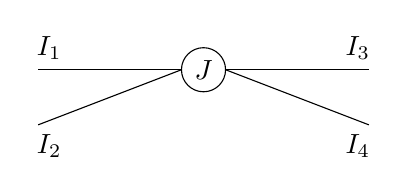
\begin{tikzpicture}[scale=1.4]
\draw (-1.5,0)--(-0.2,0);
\draw (0,0) circle (0.2);
\draw (0.2,0)--(1.5,0);
\draw (-0.2,0)--(-1.5,-0.5);
\draw (0.2,0)--(1.5,-0.5);
\node at (0,0) {$J$};
\node [above] at (-1.4,0) {$I_1$};
\node [above] at (1.4,0) {$I_3$};
\node [below] at (-1.4,-0.5) {$I_2$};
\node [below] at (1.4,-0.5) {$I_4$};
\end{tikzpicture}
\caption{Generic 2x2 junction.}
\label{fig:junction}
\end{figure}
	
\begin{itemize}
	\item $I_i=[a_i,b_i]$ for $i=1,2$ and $I_j=[a_j,b_j]$ for $j=3,4$.
	\item $\del_t \rho +\del_x f(\rho)=0$ holds on each $I_i$ and $I_j$.
	\item Flux function strictly concave.
	\item $f(0)=f(1)=0$.
	\item Flux function has a unique maximum at $\rho^{cr} \in ]0,1[$.
\end{itemize}
\end{frame}

%\subsubsection{Junction assumptions}
\begin{frame}
	\frametitle{Junction assumptions}
\begin{enumerate} 
	\item A traffic distribution matrix is given \[
 A = \begin{bmatrix}
       \alpha_{3,1} & \alpha_{3,2}            \\[0.3em]
       \alpha_{4,1} & \alpha_{4,2}
     \end{bmatrix}
\]
\textcolor{red}{Remark:} $\alpha_{j,1}\neq\alpha_{j,2} \quad \forall j\in\left\lbrace3,4\right\rbrace.$
	\item Rankine-Hugoniot condition is satisfied, i.e., $$\sum_{i=1}^2 f_i(\rho(t,b_i-))=\sum_{j=3}^4 f_j(\rho(t,a_j+)).$$
	\item \label{item:cons_flux} Each $f_j(\rho(t,a_j+))=\sum\limits_{i=1}^2 \alpha_{j,i}f_i(\rho(t, b_i-))$ for every $j=3,4 .$
	\item $\sum\limits_{i=1}^2 f_i(\rho(t,b_i-))$	is maximum subject to \ref{item:cons_flux}. 
	
\end{enumerate}
	
\end{frame}

%\subsubsection{Riemann Problem at the Junction}
\begin{frame}
	\frametitle{Riemann Problem at the Junction}
\begin{itemize}
	\item Define initial data $\rho_{i,0},\rho_{j,0} \in ]0,1[$ for every $i=1,2$ and $j=3,4$.
	\vspace*{5mm}
	\item The Riemann Problem at J is the LWR where the initial conditions are given by $\rho_{i,0}(x)\equiv \rho_{i,0} $ in $I_i$ for every $i=1,2$ and $\rho_{j,0}(x)\equiv \rho_{j,0} $ in $I_j$ for every $j=3,4$.
	\vspace*{5mm}
	\item The Riemann Solver $\RS$ is the right continuous map $(t,x)\rightarrow \RS (\rho_l , \rho_r)(\frac{x}{t})$ that is the standard weak entropy solution to \eqref{eq:RP}.
\end{itemize}
\end{frame}	


%\subsubsection{Riemann Solver}
\begin{frame}[fragile]
	\frametitle{Riemann Solver}
To find a solution of the problem we will take the following steps.
\begin{itemize}
	\item Define $\gamma_1=f_1(\rho(t,b_1-))$ and $\gamma_2=f_2(\rho(t,b_2-))$.
	\item<1-> Define the space $(\gamma_1 ,\gamma_2).$
	\only<1-1> {\begin{figure}[ht]
\centering
\begin{tikzpicture}
	\draw[<->] (0,3) -- (0,0) --(2.5,0);
	\node (below) at (2.4,-0.3) {$\gamma_1$};
	\node (left) at (-0.2,2.8) {$\gamma_2$};
\end{tikzpicture}

%\caption{Solution of the Riemann Problem.}
\label{fig:spaceSet}
\end{figure}} 	
	\item<2-> Define $\gamma_i^{\max}(\rho_{i,0})$ and $\gamma_j^{\max}(\rho_{j,0})$ for each $i=1,2$ and $j=3,4$ as the maximum flux that can be obtained by a simple wave solution on each road.
	\only<2-2>{\vspace*{35mm}}
	\item<3-> Define the sets $\Omega_i=[0,\gamma_i^{\max}(\rho_{i,0})] \quad i=1,2.$
	\only<3-3>{ \begin{figure}[ht]
\centering
\begin{tikzpicture}[scale=0.5]
	\draw[<->] (0,6) -- (0,0) --(5,0);
	\draw (0,0) rectangle (2,3);
	\draw [red](2,0) -- (2,3);
	\draw [red](0,3) -- (2,3);
	\node (below) at (4.9,-0.7) {$\gamma_1$};
	\node (below) at (2.1,-0.5) {$\gamma_1^{\max}$};
	\node (left) at (-0.4,5.7) {$\gamma_2$};
	\node (left) at (-0.75,3) {$\gamma_2^{\max}$};
\end{tikzpicture}

%\caption{Solution of the Riemann Problem.}
\label{fig:Set}
\end{figure}}
\end{itemize}	
\end{frame}	


%\subsubsection{Riemann Solver II}
\begin{frame}[fragile]
	\frametitle{Riemann Solver II}
	\begin{itemize}
	\item<1-> Define the set $\Omega_j=[0,\gamma_j^{\max}(\rho_{j,0})] \quad j=3,4.$
	\only<1-1> { \begin{figure}[ht]
\centering
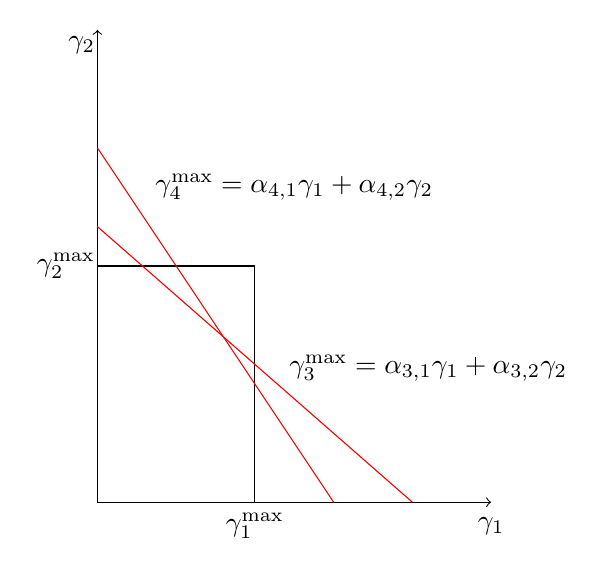
\begin{tikzpicture}
	\draw[<->] (0,6) -- (0,0) --(5,0);
	\draw (0,0) rectangle (2,3);
	\draw [red](3,0) -- (0,4.5);
	\draw [red](0,3.5) --(4,0);
	\node (below) at (5,-0.3) {$\gamma_1$};
	\node (below) at (2,-0.3) {$\gamma_1^{\max}$};
	\node (left) at (-0.2,5.8) {$\gamma_2$};
	\node (left) at (-0.4,3) {$\gamma_2^{\max}$};
	\node (right) at (4.2,1.7) {$\gamma_3^{\max}=\alpha_{3,1}\gamma_1+\alpha_{3,2}\gamma_2$};
	\node (right) at (2.5,4) {$\gamma_4^{\max}=\alpha_{4,1}\gamma_1+\alpha_{4,2}\gamma_2$};
\end{tikzpicture}

%\caption{Solution of the Riemann Problem.}
\label{fig:omegaj}
\end{figure}}
	\item<2-> Define the set $\Omega=\left\lbrace(\gamma_1,\gamma_2)\in \Omega_1\times \Omega_2 \mid A\cdot (\gamma_1 , \gamma_2)^{T}\in \Omega_3\times\Omega_4\right\rbrace .$
	\only<2-3> { \begin{figure}[ht]
\centering
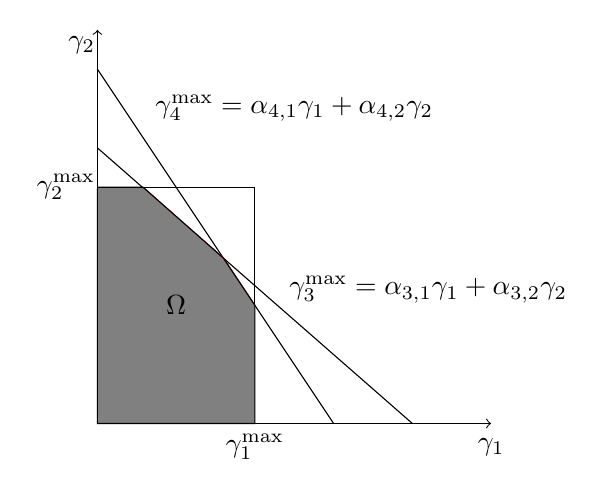
\begin{tikzpicture}
	\draw[<->] (0,5) -- (0,0) --(5,0);
	\draw (0,0) rectangle (2,3);
	\draw (3,0) -- (0,4.5);
	\draw (0,3.5) --(4,0);
	\draw [red](0,3) -- (0.58,3);
	\draw [red](1.6,2.1) -- (0.58,3);
	\draw [red](1.6,2.1) -- (2,1.5);
	\draw [red](2,0) -- (2,1.5);
	\draw[fill=gray] (0,0)--(0,3) to (0,0) -- (2,0) to (2,0)--(2,1.5) to (2, 1.5)--(1.6,2.1) to (1.6,2.1)--(0.58,3) to (0.58,3)--(0,3) ;
	\node (below) at (5,-0.3) {$\gamma_1$};
	\node (below) at (2,-0.3) {$\gamma_1^{\max}$};
	\node (left) at (-0.2,4.8) {$\gamma_2$};
	\node (left) at (-0.4,3) {$\gamma_2^{\max}$};
	\node (right) at (4.2,1.7) {$\gamma_3^{\max}=\alpha_{3,1}\gamma_1+\alpha_{3,2}\gamma_2$};
	\node (right) at (2.5,4) {$\gamma_4^{\max}=\alpha_{4,1}\gamma_1+\alpha_{4,2}\gamma_2$};
	\node (above) at (1,1.5) {$\Omega$};
\end{tikzpicture}
%\caption{Solution of the Riemann Problem.}
\label{fig:omega}
\end{figure}}
\item<3-> The set $\Omega$ is closed, convex and not empty.
\item<4->\textcolor{red}{Unique solution:}
\begin{figure}[ht]
\centering
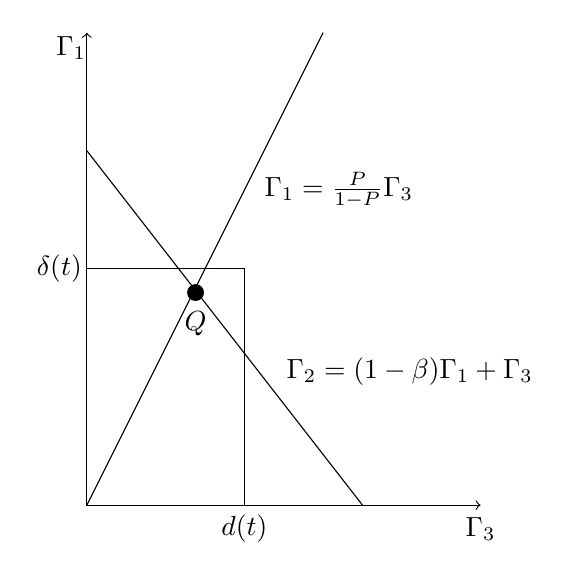
\begin{tikzpicture}
	\draw[<->] (0,6) -- (0,0) --(5,0);
	\draw (0,0) rectangle (2,3);
	\draw (3.5,0) -- (0,4.5);
	\draw (0,0) -- (1,2)--(3,6);
	\draw[fill=black](1.38,2.7) circle (0.1);
	\node (below) at (5,-0.3) {$\Gamma_3$};
	\node (below) at (2,-0.3) {$d(t)$};
	\node (left) at (-0.2,5.8) {$\Gamma_1$};
	\node (left) at (-0.35,3) {$\delta(t)$};
	\node (right) at (4.1,1.7) {$\Gamma_2=(1-\beta)\Gamma_1 +\Gamma_3$};
	\node (right) at (3.2,4) {$\Gamma_1=\frac{P}{1-P}\Gamma_3$};
	\node (below) at (1.38,2.3) {$Q$};
\end{tikzpicture}

%\caption{Solution of the Riemann Problem.}
\label{fig:solution}
\end{figure}
\end{itemize}
\end{frame}

%\subsection{2x1 Junction model}
\subsubsection{2x1 Junction Solution}
\begin{frame}[fragile]
	\frametitle{2x1 Junction Solution}
	\begin{center}
\textcolor{red}{What happens if we have a 2x1 junction?}
	\end{center}
\pause	
	\begin{figure}[ht]
\centering
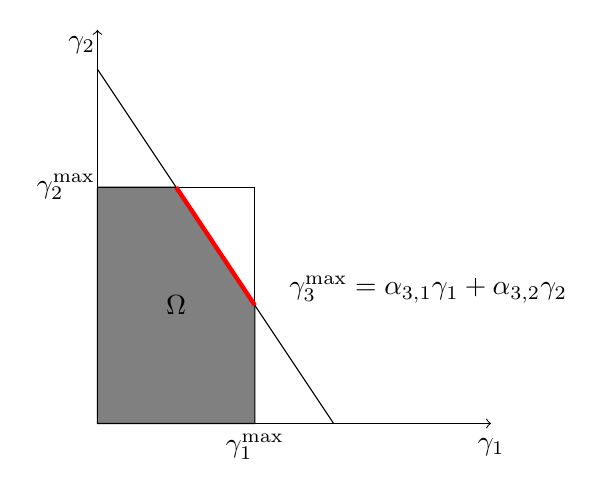
\begin{tikzpicture}
	\draw[<->] (0,5) -- (0,0) --(5,0);
	\draw (0,0) rectangle (2,3);
	\draw (3,0) -- (0,4.5);
	\draw[fill=gray] (0,0)--(0,3) to (0,0) -- (2,0) to (2,0)--(2,1.5) to (2, 1.5)--(1,3) to (0.58,3)--(0,3) ;
	\draw [ultra thick, red] (1,3)--(2,1.5);
	\node (below) at (5,-0.3) {$\gamma_1$};
	\node (below) at (2,-0.3) {$\gamma_1^{\max}$};
	\node (left) at (-0.2,4.8) {$\gamma_2$};
	\node (left) at (-0.4,3) {$\gamma_2^{\max}$};
	\node (right) at (4.2,1.7) {$\gamma_3^{\max}=\alpha_{3,1}\gamma_1+\alpha_{3,2}\gamma_2$};
	\node (above) at (1,1.5) {$\Omega$};
\end{tikzpicture}
%\caption{Solution of the Riemann Problem.}
\label{fig:2x1junction}
\end{figure}
\pause
\begin{center}
\textbf{The solution is not unique!}
\end{center}
\end{frame}

%\subsubsection{Assumptions}
\begin{frame}[fragile]
	\frametitle{Assumptions}
\begin{itemize}
	\item Introduce a priority parameter $P \in ]0,1[$.
	\vspace*{5mm}
	\item In the outgoing road, $Pf_1(\rho_1(t,b_1+))$ will be the portion of flux coming from the first incoming road, and $(1-P)f_2(\rho_2(t,b_2+))$, the one coming from the second. 
	\vspace*{5mm}	
	\item To maximize the traffic going through, we set $$\hat{\gamma}_3=\min{\left\lbrace\gamma_1^{\max}(\rho_{1,0})+\gamma_2^{\max}(\rho_{2,0}),\gamma_3^{\max}(\rho_{3,0})\right\rbrace} .$$
	
\end{itemize}

\end{frame}

%\subsubsection{Riemann Solver}
\begin{frame}[fragile]
	\frametitle{Riemann Solver}
	\begin{itemize}
	\item<1-> We follow all the steps as in the other case and what we obtain is $\Omega=\left\lbrace (\gamma_1,\gamma_2): 0\leq\gamma_i\leq\gamma_i^{max}(\rho_{i,0}), 0\leq\gamma_1+\gamma_2\leq\hat{\gamma}_3\right\rbrace .$
	\only<1-1>{	\begin{figure}[ht]
\centering
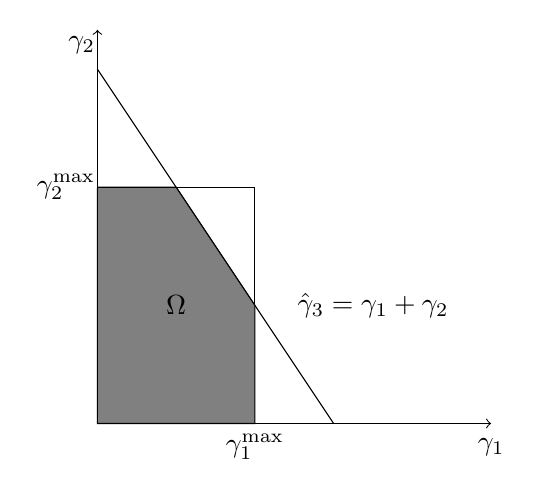
\begin{tikzpicture}
	\draw[<->] (0,5) -- (0,0) --(5,0);
	\draw (0,0) rectangle (2,3);
	\draw (3,0) -- (0,4.5);
	\draw[fill=gray] (0,0)--(0,3) to (0,0) -- (2,0) to (2,0)--(2,1.5) to (2, 1.5)--(1,3) to (0.58,3)--(0,3) ;
	%\draw [ultra thick, red] (1,3)--(2,1.5);
	\node (below) at (5,-0.3) {$\gamma_1$};
	\node (below) at (2,-0.3) {$\gamma_1^{\max}$};
	\node (left) at (-0.2,4.8) {$\gamma_2$};
	\node (left) at (-0.4,3) {$\gamma_2^{\max}$};
	\node (right) at (3.5,1.5) {$\hat{\gamma}_3=\gamma_1+\gamma_2$};
	\node (above) at (1,1.5) {$\Omega$};
\end{tikzpicture}
%\caption{Solution of the Riemann Problem.}
\label{fig:2x1juncSol}
\end{figure}}
	\item<2-> We draw the line $\gamma_2=\dfrac{P}{1-P}\gamma_1 .$
	\only<2-2>	{\begin{figure}[ht]
\centering
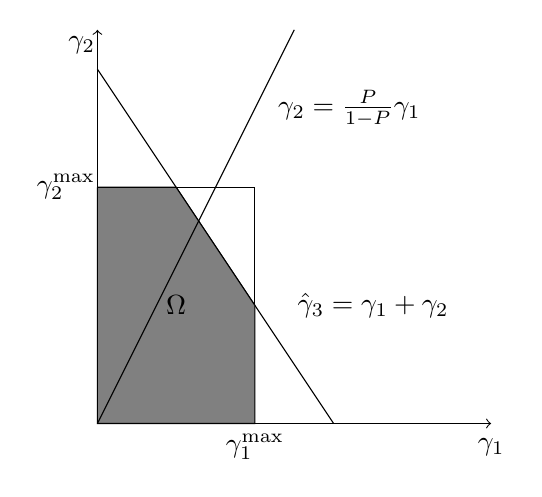
\begin{tikzpicture}
	\draw[<->] (0,5) -- (0,0) --(5,0);
	\draw (0,0) rectangle (2,3);
	\draw (3,0) -- (0,4.5);
	\draw[fill=gray] (0,0)--(0,3) to (0,0) -- (2,0) to (2,0)--(2,1.5) to (2, 1.5)--(1,3) to (0.58,3)--(0,3) ;
	\draw (0,0) -- (1,2)--(2.5,5);
	%\draw[ultra thick, red](1.3,2.58) circle (0.1);
	\node (below) at (5,-0.3) {$\gamma_1$};
	\node (below) at (2,-0.3) {$\gamma_1^{\max}$};
	\node (left) at (-0.2,4.8) {$\gamma_2$};
	\node (left) at (-0.4,3) {$\gamma_2^{\max}$};
	\node (right) at (3.5,1.5) {$\hat{\gamma}_3=\gamma_1+\gamma_2$};
	\node (above) at (1,1.5) {$\Omega$};
	\node (right) at (3.2,4) {$\gamma_2=\frac{P}{1-P}\gamma_1$};
	%\node (below) at (1.3,2.1) {$Q$};
\end{tikzpicture}
%\caption{Solution of the Riemann Problem.}
\label{fig:2x1juncPrior}
\end{figure}}
	\item<3-> Three cases: 
	\vspace*{5mm}
	\only<3-3>{\begin{columns}
	\column{0.33 \textwidth}
	\begin{figure}[ht]
\centering
{
\resizebox{.9\columnwidth}{!}{
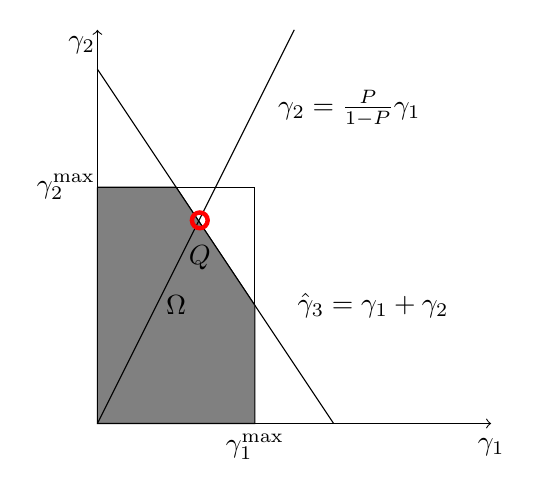
\begin{tikzpicture}
	\draw[<->] (0,5) -- (0,0) --(5,0);
	\draw (0,0) rectangle (2,3);
	\draw (3,0) -- (0,4.5);
	\draw[fill=gray] (0,0)--(0,3) to (0,0) -- (2,0) to (2,0)--(2,1.5) to (2, 1.5)--(1,3) to (0.58,3)--(0,3) ;
	\draw (0,0) -- (1,2)--(2.5,5);
	\draw[ultra thick, red](1.3,2.58) circle (0.1);
	\node (below) at (5,-0.3) {$\gamma_1$};
	\node (below) at (2,-0.3) {$\gamma_1^{\max}$};
	\node (left) at (-0.2,4.8) {$\gamma_2$};
	\node (left) at (-0.4,3) {$\gamma_2^{\max}$};
	\node (right) at (3.5,1.5) {$\hat{\gamma}_3=\gamma_1+\gamma_2$};
	\node (above) at (1,1.5) {$\Omega$};
	\node (right) at (3.2,4) {$\gamma_2=\frac{P}{1-P}\gamma_1$};
	\node (below) at (1.3,2.1) {$Q$};
\end{tikzpicture}}
%\caption{Solution of the Riemann Problem.}
\label{fig:2x1juncSolIns}}
\end{figure}
	\column{0.33 \textwidth}
	\begin{figure}[ht]
\centering
{
\resizebox{.9\columnwidth}{!}{
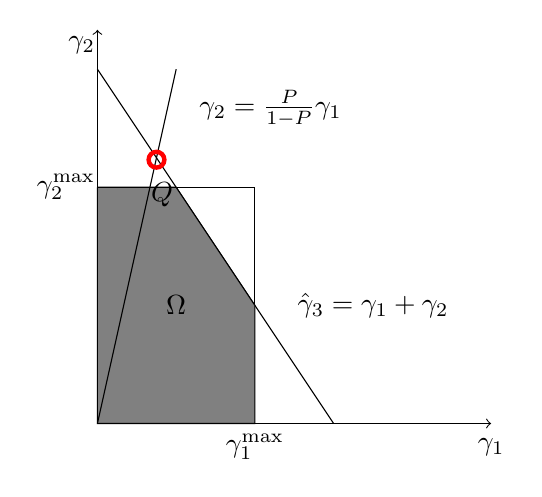
\begin{tikzpicture}
	\draw[<->] (0,5) -- (0,0) --(5,0);
	\draw (0,0) rectangle (2,3);
	\draw (3,0) -- (0,4.5);
	\draw[fill=gray] (0,0)--(0,3) to (0,0) -- (2,0) to (2,0)--(2,1.5) to (2, 1.5)--(1,3) to (0.58,3)--(0,3) ;
	\draw (0,0) -- (1,4.5);
	\draw[ultra thick, red](0.75,3.35) circle (0.1);
	\node (below) at (5,-0.3) {$\gamma_1$};
	\node (below) at (2,-0.3) {$\gamma_1^{\max}$};
	\node (left) at (-0.2,4.8) {$\gamma_2$};
	\node (left) at (-0.4,3) {$\gamma_2^{\max}$};
	\node (right) at (3.5,1.5) {$\hat{\gamma}_3=\gamma_1+\gamma_2$};
	\node (above) at (1,1.5) {$\Omega$};
	\node (right) at (2.2,4) {$\gamma_2=\frac{P}{1-P}\gamma_1$};
	\node (below) at (0.82,2.9) {$Q$};
\end{tikzpicture}}
%\caption{Solution of the Riemann Problem.}
\label{fig:2x1juncSolOut1}}
\end{figure}
	\column{0.33 \textwidth}
	\begin{figure}[ht]
\centering
{
\resizebox{.9\columnwidth}{!}{
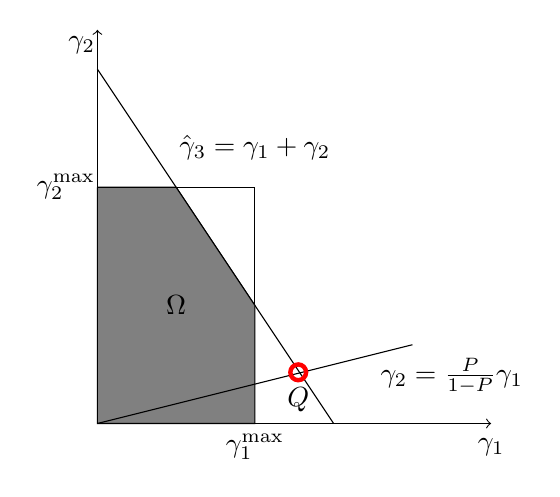
\begin{tikzpicture}
	\draw[<->] (0,5) -- (0,0) --(5,0);
	\draw (0,0) rectangle (2,3);
	\draw (3,0) -- (0,4.5);
	\draw[fill=gray] (0,0)--(0,3) to (0,0) -- (2,0) to (2,0)--(2,1.5) to (2, 1.5)--(1,3) to (0.58,3)--(0,3) ;
	\draw (0,0) -- (4,1);
	\draw[ultra thick, red](2.55,0.65) circle (0.1);
	\node (below) at (5,-0.3) {$\gamma_1$};
	\node (below) at (2,-0.3) {$\gamma_1^{\max}$};
	\node (left) at (-0.2,4.8) {$\gamma_2$};
	\node (left) at (-0.4,3) {$\gamma_2^{\max}$};
	\node (right) at (2,3.5) {$\hat{\gamma}_3=\gamma_1+\gamma_2$};
	\node (above) at (1,1.5) {$\Omega$};
	\node (right) at (4.5,0.6) {$\gamma_2=\frac{P}{1-P}\gamma_1$};
	\node (below) at (2.55,0.3) {$Q$};
\end{tikzpicture}}
%\caption{Solution of the Riemann Problem.}
\label{fig:2x1juncSolOut2}}
\end{figure}
\end{columns}
	}
	\end{itemize}

\end{frame}

%\subsubsection{Riemann Solver II}
\begin{frame}[fragile]
	\frametitle{Riemann Solver II}
	\begin{itemize}
	\item<1-> If $Q\in \Omega$ then $Q$ is the solution.
	\only<1-1> {	\begin{figure}[ht]
\centering
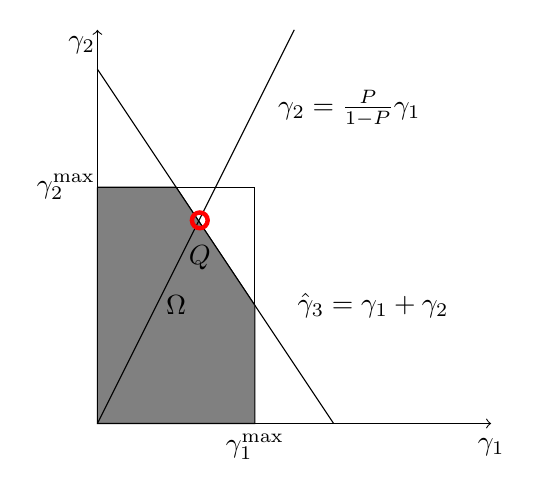
\begin{tikzpicture}
	\draw[<->] (0,5) -- (0,0) --(5,0);
	\draw (0,0) rectangle (2,3);
	\draw (3,0) -- (0,4.5);
	\draw[fill=gray] (0,0)--(0,3) to (0,0) -- (2,0) to (2,0)--(2,1.5) to (2, 1.5)--(1,3) to (0.58,3)--(0,3) ;
	\draw (0,0) -- (1,2)--(2.5,5);
	\draw[ultra thick, red](1.3,2.58) circle (0.1);
	\node (below) at (5,-0.3) {$\gamma_1$};
	\node (below) at (2,-0.3) {$\gamma_1^{\max}$};
	\node (left) at (-0.2,4.8) {$\gamma_2$};
	\node (left) at (-0.4,3) {$\gamma_2^{\max}$};
	\node (right) at (3.5,1.5) {$\hat{\gamma}_3=\gamma_1+\gamma_2$};
	\node (above) at (1,1.5) {$\Omega$};
	\node (right) at (3.2,4) {$\gamma_2=\frac{P}{1-P}\gamma_1$};
	\node (below) at (1.3,2.1) {$Q$};
\end{tikzpicture}
%\caption{Solution of the Riemann Problem.}
\label{fig:Inside}
\end{figure}}
	\item<2-> If $Q \notin\Omega$ we set a point $P$ such that $P\in \Omega \cap \left\lbrace (\gamma_1,\gamma_2):\gamma_1+\gamma_2=\hat{\gamma}_3\right\rbrace $ closest to priority line.
	\only<2-2> {\begin{columns}
	\column{0.5 \textwidth}
	\begin{figure}[ht]
\centering
{
\resizebox{.9\columnwidth}{!}{
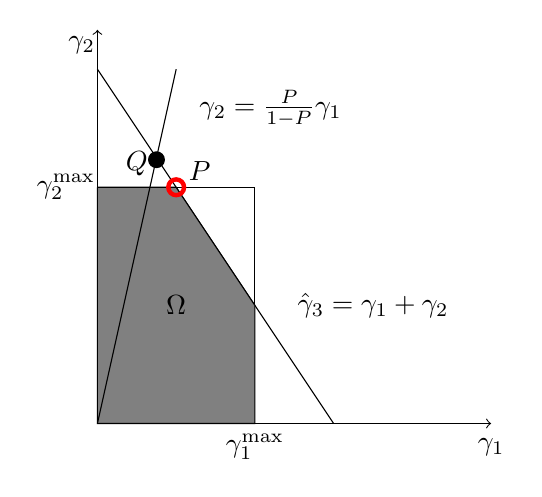
\begin{tikzpicture}
	\draw[<->] (0,5) -- (0,0) --(5,0);
	\draw (0,0) rectangle (2,3);
	\draw (3,0) -- (0,4.5);
	\draw[fill=gray] (0,0)--(0,3) to (0,0) -- (2,0) to (2,0)--(2,1.5) to (2, 1.5)--(1,3) to (0.58,3)--(0,3) ;
	\draw (0,0) -- (1,4.5);
	\draw[fill=black](0.75,3.35) circle (0.1);
	\draw[ultra thick, red](1,3) circle (0.1);
	\node (below) at (5,-0.3) {$\gamma_1$};
	\node (below) at (2,-0.3) {$\gamma_1^{\max}$};
	\node (left) at (-0.2,4.8) {$\gamma_2$};
	\node (left) at (-0.4,3) {$\gamma_2^{\max}$};
	\node (right) at (3.5,1.5) {$\hat{\gamma}_3=\gamma_1+\gamma_2$};
	\node (above) at (1,1.5) {$\Omega$};
	\node (right) at (2.2,4) {$\gamma_2=\frac{P}{1-P}\gamma_1$};
	\node (left) at (0.5,3.3) {$Q$};
	\node (right) at (1.3,3.2) {$P$};
\end{tikzpicture}}
%\caption{Solution of the Riemann Problem.}
\label{fig:P1}}
\end{figure}
	\column{0.5 \textwidth}
	\begin{figure}[ht]
\centering
{
\resizebox{.9\columnwidth}{!}{
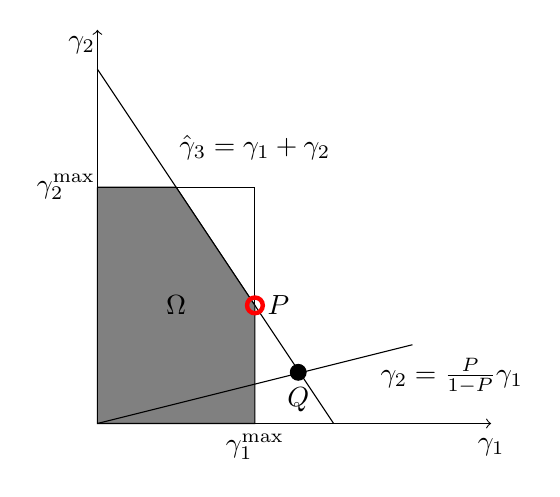
\begin{tikzpicture}
	\draw[<->] (0,5) -- (0,0) --(5,0);
	\draw (0,0) rectangle (2,3);
	\draw (3,0) -- (0,4.5);
	\draw[fill=gray] (0,0)--(0,3) to (0,0) -- (2,0) to (2,0)--(2,1.5) to (2, 1.5)--(1,3) to (0.58,3)--(0,3) ;
	\draw (0,0) -- (4,1);
	\draw[fill=black](2.55,0.65) circle (0.1);
	\draw[ultra thick, red](2,1.5) circle (0.1);
	\node (below) at (5,-0.3) {$\gamma_1$};
	\node (below) at (2,-0.3) {$\gamma_1^{\max}$};
	\node (left) at (-0.2,4.8) {$\gamma_2$};
	\node (left) at (-0.4,3) {$\gamma_2^{\max}$};
	\node (right) at (2,3.5) {$\hat{\gamma}_3=\gamma_1+\gamma_2$};
	\node (above) at (1,1.5) {$\Omega$};
	\node (right) at (4.5,0.6) {$\gamma_2=\frac{P}{1-P}\gamma_1$};
	\node (below) at (2.55,0.3) {$Q$};
	\node (right) at (2.3,1.5) {$P$};
\end{tikzpicture}}
%\caption{Solution of the Riemann Problem.}
\label{fig:Ppoint2}}
\end{figure}
\end{columns}
	}
	\end{itemize}
\end{frame}	

%\subsubsection{Riemann Solver III}
\begin{frame}[fragile]
	\frametitle{Riemann Solver III}
The solutions we found are in the flux domain. How to go back to the density domain?
\begin{definition}
Let $\tau:[0,1]\rightarrow[0,1]$ be the map such that:
	\begin{itemize}
		\item $f(\tau(\rho))=f(\rho)$ for every $\rho\in [0,1]$;
		\item $\tau(\rho)\neq\rho$ for every $\rho\in[0,1]\setminus\{\rho^{cr}\}.$
	\end{itemize}
\end{definition}	
The function $\tau(\rho)$ is continuous and well defined. Moreover, it satisfies $$0\leq\rho\leq\rho^{cr}  \Longleftrightarrow \rho^{cr}\leq\tau(\rho)\leq 1 \qquad 0\leq\tau(\rho)\leq\rho^{cr}  \Longleftrightarrow \rho^{cr}\leq\rho\leq 1.$$
\end{frame}

%\subsubsection{Riemann Solver IV}
\begin{frame}[label=Solution,fragile]
	\frametitle{Riemann Solver IV}
Given $\rho_i(0,\cdot), \rho_j(0,\cdot) \; \text{for every}\; i,j$ there exists a $n+m$-tuple $(\hat{\rho}_i ,\hat{\rho}_j)\in[0,1]^{n+m}$ such that
	\begin{equation}
		\hat{\rho}_i\in\left\{
		\begin{array}{ll}
		\{\rho_{i,0}\}\cup]\tau(\rho_{i,0}),1] &\hbox{if}~0 \leq \rho_{i,0}\leq\rho^{cr} ,\\
		\left[\rho^{cr},1\right] &\hbox{if}~\rho^{cr} \leq \rho_{i,0}\leq 1;
		\end{array}
		\right.
		\label{eq:rho_i}
		\hyperlink{drawing}{\beamerbutton{...}}
	\end{equation}
	and
	\begin{equation}
		\hat{\rho}_j\in\left\{
		\begin{array}{ll}
		\left[0,\rho^{cr}\right] &\hbox{if}~0 \leq \rho_{j,0}\leq\rho^{cr} ,\\		
		\{\rho_{j,0}\}\cup[0,\tau(\rho_{j,0})[ &\hbox{if}~\rho^{cr} \leq \rho_{j,0}\leq 1;
		\end{array}
		\right.
		\label{eq:rho_j}
		\hyperlink{drawingO}{\beamerbutton{...}}
	\end{equation}
and for the incoming roads the solutions are given by the waves $(\rho_{i,0},\hat{\rho}_i)$, while for the outgoing road the solutions are given by the waves $(\hat{\rho}_j,\rho_{j,0})$ for every $i,j$.\\

\begin{flushright}
\hyperlink{Theorem}{\beamerbutton{Theorem}}
\end{flushright}
\end{frame}

%\subsubsection{Riemann Solver V}
\begin{frame}[label=drawing, fragile]
	\frametitle{Riemann Solver V}
For the incoming roads
\only<1->{\begin{columns}
	\column{0.5 \textwidth}
	\begin{figure}[ht]
\centering
{
\resizebox{.9\columnwidth}{!}{
\begin{tikzpicture}[scale=1.4]
\draw [<->](0,3.5)--(0,0) -- (5,0);
\draw (0,0) .. controls (1,3) and (2,4) .. (4,0);
\draw[fill=black](0.73,1.8) circle (0.05);
\draw[ultra thick](4,0)..controls (3.5,0.95) .. (2.93,1.8);
\draw[fill=black](3.5,0.95) circle (0.05);
%\draw (0,0) .. controls (1,3) and (2.5,1) .. (3,0);
%\draw (0,1)--(2.5,2.28);
%\draw (0,0) -- (1,0.52)--(3.08,1.6);
\draw [ ultra thick, red] (0.73,1.8)--(3.5,0.95);
\draw [dashed] (0.73,0)--(0.73,1.8); 
\draw [dashed] (0.73,1.8)--(2.9,1.8);
\draw [dashed] (3.5,0)--(3.5,0.95);
\node [below] at (4.9,0) {$\rho$};
\node [left] at (0,3.3) {$f(\rho)$};
%\node [below] at (3.1,0.08) {$\rho^*$};
\node (above) at (2,1.6) {S};
\node [below] at (3.5,0.05) {$\hat{\rho}_{i}$};
\node [below] at (0.73,0) {$\rho_{i,0}$};
%\node [above] at (1.5,1.71) {$V_b$};
\end{tikzpicture}}
%\caption{Solution of the Riemann Problem.}
\label{fig:I1}}
\end{figure}
	\column{0.5 \textwidth}
	\begin{figure}[ht]
\centering
{
\resizebox{.9\columnwidth}{!}{
\begin{tikzpicture}[scale=1.4]
\draw [<->](0,3.5)--(0,0) -- (5,0);
\draw (0,0) .. controls (1,3) and (2,4) .. (4,0);
%\draw[fill=black](0.73,1.8) circle (0.05);
\draw[ultra thick](4,0)..controls (3.5,0.95) and (2.7,2.77) .. (1.6,2.6);
\draw[fill=black](3.5,0.95) circle (0.05);
%\draw (0,0) .. controls (1,3) and (2.5,1) .. (3,0);
%\draw (0,1)--(2.5,2.28);
%\draw (0,0) -- (1,0.52)--(3.08,1.6);
%\draw [ ultra thick, red] (0.73,1.8)--(3.5,0.95);
%\draw [dashed] (0.73,0)--(0.73,1.8); 
%\draw [dashed] (0.73,1.8)--(2.9,1.8);
\node (above) at (3.2,2) {R};
\node (above) at (4,0.5) {S};
\draw [dashed] (3.5,0)--(3.5,0.95);
\node [below] at (4.9,0) {$\rho$};
\node [left] at (0,3.3) {$f(\rho)$};
%\node [below] at (3.1,0.08) {$\rho^*$};
\node [below] at (3.5,0.0) {$\rho_{i,0}$};
%\node [below] at (0.73,0) {$\rho_{i,0}$};
%\node [above] at (1.5,1.71) {$V_b$};
\end{tikzpicture}}
%\caption{Solution of the Riemann Problem.}
\label{fig:I2}}
\end{figure}
\end{columns}
\begin{flushright}
\hyperlink{Solution}{\beamerbutton{Back}}
\end{flushright}	}
\end{frame}


%\subsubsection{Riemann Solver Vbis}

\begin{frame}[label=drawingO, fragile]
\frametitle{Riemann Solver V}
For the outgoing roads	
\begin{columns}
	\column{0.5 \textwidth}
	\begin{figure}[ht]
\centering
{
\resizebox{.9\columnwidth}{!}{
\begin{tikzpicture}[scale=1.4]
\draw [<->](0,3.5)--(0,0) -- (5,0);
\draw (0,0) .. controls (1,3) and (2,4) .. (4,0);
%\draw[fill=black](0.73,1.8) circle (0.05);
\draw[ultra thick](0,0)..controls (0.35,0.95) and (0.85,2.38) .. (1.6,2.6);
\draw[fill=black](0.35,0.95) circle (0.05);
%\draw (0,0) .. controls (1,3) and (2.5,1) .. (3,0);
%\draw (0,1)--(2.5,2.28);
%\draw (0,0) -- (1,0.52)--(3.08,1.6);
%\draw [ ultra thick, red] (0.73,1.8)--(3.5,0.95);
%\draw [dashed] (0.73,0)--(0.73,1.8); 
%\draw [dashed] (0.73,1.8)--(2.9,1.8);
\node (above) at (0.4,1.5) {R};
\node (above) at (0.1,0.6) {S};
\draw [dashed] (0.35,0)--(0.35,0.95);
\node [below] at (4.9,0) {$\rho$};
\node [left] at (0,3.3) {$f(\rho)$};
%\node [below] at (3.1,0.08) {$\rho^*$};
\node [below] at (0.35,0.0) {$\rho_{j,0}$};
%\node [below] at (0.73,0) {$\rho_{i,0}$};
%\node [above] at (1.5,1.71) {$V_b$};
\end{tikzpicture}}
%\caption{Solution of the Riemann Problem.}
\label{fig:I1}}
\end{figure}
	\column{0.5 \textwidth}
	\begin{figure}[ht]
\centering
{
\resizebox{.9\columnwidth}{!}{
\begin{tikzpicture}[scale=1.4]
\draw [<->](0,3.5)--(0,0) -- (5,0);
\draw (0,0) .. controls (1,3) and (2,4) .. (4,0);
\draw[fill=black](2.95,1.8) circle (0.05);
\draw[ultra thick](0,0)..controls (0.35,0.95) .. (0.73,1.8);
\draw[fill=black](0.35,0.95) circle (0.05);
%\draw (0,0) .. controls (1,3) and (2.5,1) .. (3,0);
%\draw (0,1)--(2.5,2.28);
%\draw (0,0) -- (1,0.52)--(3.08,1.6);
\node (above) at (1.5,1.5) {S};
\draw [ ultra thick, red] (0.35,0.95)--(2.95,1.8);
\draw [dashed] (2.95,0)--(2.95,1.8); 
\draw [dashed] (0.73,1.8)--(2.9,1.8);
\draw [dashed] (0.35,0)--(0.35,0.95);
\node [below] at (4.9,0) {$\rho$};
\node [left] at (0,3.3) {$f(\rho)$};
%\node [below] at (3.1,0.08) {$\rho^*$};
\node [below] at (0.35,0.05) {$\hat{\rho}_{j}$};
\node [below] at (2.95,0) {$\rho_{j,0}$};
%\node [above] at (1.5,1.71) {$V_b$};
\end{tikzpicture}}
%\caption{Solution of the Riemann Problem.}
\label{fig:O2}}
\end{figure}
\end{columns}
\begin{flushright}
\hyperlink{Solution}{\beamerbutton{Back}}
\end{flushright}	
	
\end{frame}

%\subsubsection{Self-similarity}
\begin{frame}[label=Theorem, fragile]
\frametitle{Self-similarity}
\begin{theorem}
	\label{th:existenceSolPiccoli}
	Consider a junction $J$ and a priority parameter $P\in ]0,1[$ or a distribution matrix $A$. Then there exists a unique Riemann Solver $\RS$ such that for a.e. $t>0$ it holds 
	$$(\rho_i(t,b_i-),\rho_j(t,a_j+))=\RS(\rho_i(t,b_i-),\rho_j(t,a_j+)) \quad \forall i,j .$$ 
\end{theorem}
\end{frame}

\frame{
  \setbeamercovered{transparent}
	\frametitle{Self-similarity and LN-CTM~\cite{Muralidharana}}
  \begin{itemize}
    \item<1-> Self-similarity: guarantees junction solution only generates one shock
    \item<2-> Subsequent solutions of junction should be stationary, assuming Riemann conditions (see Figure~\ref{fig:ss})
  \end{itemize}
  \begin{figure}[ht]
\centering
{
\resizebox{.4\columnwidth}{!}{
\def \scale{1.5}
\begin{tikzpicture}[scale=\scale,domain=0:1]

\def \rampDem{1.7}
\def \rampDemPlus{1.7}
\def \dem{1.7}
\def \demPlus{2.8}
\def \priorityRat{0.6}
\def \splitRat{0.4}
\def \totalFlow{1.5}

\coordinate (Z) at (0,0);
\coordinate (I1) at (\rampDem, 0);
\coordinate (I1') at (\rampDemPlus, 0);
\coordinate (I2) at (0, \dem);
\coordinate (I2') at (0, \demPlus);
\coordinate (I3) at (\rampDem, \dem);
\coordinate (I3') at (\rampDemPlus, \demPlus);
\coordinate (A) at (0, {\totalFlow/(1-\splitRat)});
\coordinate (B) at (\totalFlow, 0);
\coordinate (C) at ({(1-\priorityRat)/\priorityRat*\dem}, \dem);
\coordinate (D) at (intersection of I2'--I3' and Z--C);


\draw[->] (Z) -- (3.5,0) node[below right]{$r_i$};
\draw[->] (Z) -- (0,4) node[left]{$f^{\text{out}}_i$};

\draw[dashed] (I3) -- (I1) node[below]{$d_i(t_0),d_i(t_0^+)$};
\draw[dashed] (I3) -- (I2) node[left]{$\delta_i(t_0)$};
\draw[dashed] (I3) -- (I1');
\draw (I3) -- (I3');
\draw (I3') -- (I2') node[left]{$\delta_i(t_0^+)$};
\draw[<->] (A) -- (B) node[yshift=1cm, xshift=0cm]{};
\draw[->, dashed, red, ultra thick] (Z) -- (I3) node[midway, xshift=1cm]{};
\draw[->, red, ultra thick] (Z) -- (I3') node[midway, xshift=1cm]{};
\draw [red, ultra thick, radius=.1, dashed] (intersection of A--B and Z--I3) circle;
\draw [red, ultra thick, radius=.1] (intersection of A--B and Z--I3') circle;

\end{tikzpicture}}
\caption{LN-CTM is not self-similar when considering the limit of the discrete model}
\label{fig:ss}}
\end{figure}
}